\section{Background and Related Work}\label{sec:network:background}

\subsection{\acrshort{UMTS} Networks and the \acrshort{RRC} Protocol}\label{sec:network:background:umts_rrc}
A \gls{3G} \gls{UMTS} mobile network consists of three main components, which are depicted in \reffig{fig:network:background:mobile_network_overview}: The \gls{UE}, the \gls{RAN}, and the \cls{CN}.
The \gls{RAN} is used to establish connectivity between the \gls{UE} and the \gls{CN}, which in turn can establish connectivity to the Internet, if required.

\gls{UE} consists of devices used by end users, i.e. smartphones, tablets or data card enabled notebooks, but can also include \gls{M2M} devices.
The \gls{RAN} is, amongst other tasks, responsible for \gls{RRC}, packet scheduling and handover control.
It includes network entities such as the \gls{NodeB} and the \gls{RNC}.
The \gls{CN} provides the backbone network of the \gls{UMTS} network and provides connectivity to the Internet and the \gls{PSTN}.
Furthermore, functionality such as billing, authentication and location management is provided by the \gls{CN}.

\begin{figure}
	\centering
	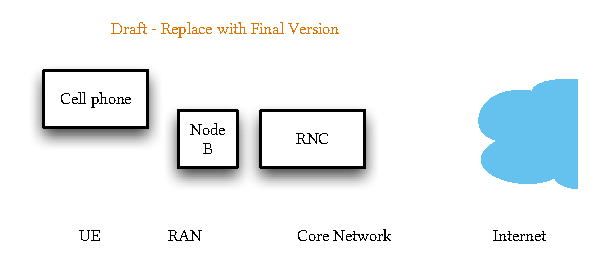
\includegraphics{network/background/figures/mobile_network_overview}
	\caption{Overview of Mobile Network}
	\label{fig:network:background:mobile_network_overview}
\end{figure}

\subsection{Measurements of \acrshort{RRC} Parameters and Optimisation of Resource Consumption}\label{sec:network:background:measurement_optimisation}

\subsection{Smartphone Energy Consumption and \acrshort{QoE}}\label{sec:network:background:energy_consumption_qoe}
